% +--------------------------------------------------------------------+
% | Sample Chapter 2
% +--------------------------------------------------------------------+

\cleardoublepage

\chapter{Criptografía y Blockchain}
\label{cap1}
%En este capitulo trataremos todo lo referente a protocolos criptograficos aplicados en blockchain.

%secciones: una breve introduccion sobre lo que se pretende con la criptografia, ecdsa: curvas elipticas, algoritmo de consenso, coste computacional de los algoritmos, quizás algun extra tipo implementacion...
%\section{Criptografía de clave pública} no poner como seccion, sino incluirlo en la introduccion del capitulo
Garantizar la autenticidad de las transacciones entre los nodos y la integridad del registro es la tarea de la criptografía dentro del blockchain. La criptografía de clave pública, donde no es necesario la existencia de un canal seguro para transmitir la información, es el método criptográfico utilizado en el Blockchain, pues justamente en este entorno público toda la información transmitida es vista por los demás participantes.
Este método, desarrollado en la década del 70 del siglo XX, solucionó algunas limitaciones de la criptografía de clave simétrica. En un entorno donde se use una misma clave tanto para cifrar como para descrifrar mensajes se debe disponer un canal seguro a través del cual esta clave sea distribuida. Existen situaciones en las que no se puede garantizar la existencia de tal canal y por tanto el uso de claves simétricas es inviable.
La criptografía de clave pública se fundamentan en la generación de una dupla $(p,q)$ donde $p$ es una clave que se transmitirá a todos los demás participantes mientras que $q$ solo será conocida por quien haya creado la dupla. A partir de $p$ es computacionalmente infactible deducir $q$ y por tanto cualquiera que haya recibido la clave pública puede usarla para cifrar un mensaje pero solo quien conozca $q$ puede determinar el mensaje original. Dentro del blockchain sin embargo el objetivo del cifrado no es ocultar información sino verificar la identidad de cada participante. Quien controle la clave privada puede usarla para firmar sus mensajes y la autenticidad de esta firma podrá ser verificada por todos aquellos que hayan recibido la clave pública. 
%ojo con esto, explicar como funciona en el blockchain y no en  una red cualquiera, mirar https://www.coindesk.com/math-behind-bitcoin/

Para especificar el principal algoritmo de clave pública usado en el blockchain (el ECDSA Elliptic Curves Digital Signature Algorithm)\citep{elliptic_cripto} y explicar con más detalle el funcionamiento del proceso de autenticación hay que definir una serie de conceptos criptográficos y algebraicos. 
\section{Curvas elípticas y ley de grupo}\label{curvas_grupo}
\theoremstyle{definition}\begin{definition}[Curva elíptica]\label{curv_ellipt}
Una curva elíptica sobre un cuerpo $\mathbb{K}$ queda definida por la ecuación \[y^2 +a_1xy+a_3 y = x^3 +a_2x^2 +a_4x +a_6\] con $a_i$ elementos del cuerpo tales que el discriminante $\Delta$ de la curva sea distinto de cero.
El discriminante de una curva elíptica viene dado por la expresión:

\begin{equation*}
  \sysdelim..\systeme{
  \Delta = -d_1^2d_4 - 8d_2^3 - 27d_3^2 + 9d_1d_2d_3,
  d_1 = a_1^2 + 4a_2,
  d_2 = 2a_4 + a_1a_3,
  d_3 = a_3^2 + 4a_6,
  d_4 = a_1^2a_6 + 4a_2a_6 - a_1a_3a_4 + a_2a_3^2 - a_4^2
  }
\end{equation*}
Con la condición $\Delta$ $\neq$ 0 garantizamos que la curva sea "suave", es decir, que no tenga ningún punto con más de una recta tangente.
\end{definition} Para los algoritmos que vamos a estudiar nos restringiremos a los casos en que $\mathbb{K}$ sea un cuerpo finito de característica $p$, con $p$ un número primo distinto de 2 o 3. Bajo estas condiciones, y haciendo un cambio de variable, la ecuación general de una curva elíptica se puede reescribir como \begin{equation} \label{elliptic}y^2 = x^3 + ax + b \end{equation} Y para que el discriminante sea distinto de cero los coeficientes $a$ y $b$ deben cumplir $4a^3 + 27b^2 \not\equiv 0(\textrm{mod}\ p)$ En lo adelante cuando se hable de una curva elíptica nos estaremos refiriendo a \ref{elliptic} sobre un cuerpo primo de característica distinta de 2 o 3, aunque para dibujar la curva o visualizar algunas operaciones debamos suponer que la tenemos definida sobre un cuerpo de característica 0 como por ejemplo $\mathbb{R}$

A los pares $(x,y)$ que cumplen \ref{elliptic} se les añade el punto del infinito y sobre esta estructura proyectiva se define la operación de suma y calculo del inverso como sigue:
\begin{description}
\item [Suma]
Dados dos puntos $P, Q$ de la curva, la recta (proyectiva) que pasa por ellos corta a la curva en otro punto (si se trata de una recta vertical se dice que corta a la curva en el punto del infinito) la reflexión de este otro punto de corte respecto del eje de las abscisas será la suma de P y Q
Un caso especial de la suma es cuando se quiere calcular P+P, en esta situación si $P =(x,y)$ con $y \not= 0$ se toma como $2P$ la reflexión respecto del eje x del punto de la corte de la tangente de P con la curva. Si $y = 0$ se toma como $2P$ el punto del infinito.
\item [Inverso]
 El inverso de un punto $P$ es el resultado de su reflexión respecto del eje de las abscisas, así, si $P$ tiene por coordenadas $(x,y)$ entonces $-P$ tendrá coordenadas $(x,-y)$
\end{description}%2P puede ser 0 pues estamos en un grupo finito??
Esta definición geométrica de las operaciones se aprecia mejor trabajando sobre los números reales, y así es como se suele representar en gráficos. En cualquier caso tal y como se hizo con el inverso, se puede dar una definición algebraica de la suma.

\begin{figure}[H]
%\centering
  \subfloat[Cálculo de $P+Q=R$]{{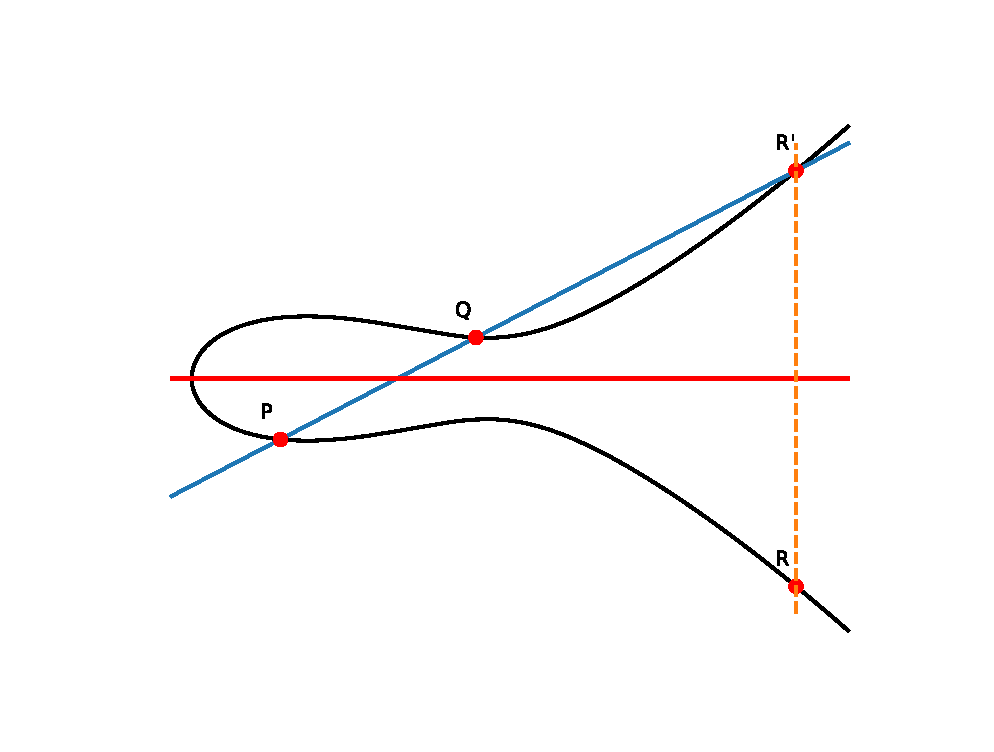
\includegraphics[width=8cm]{figures/elliptic.eps}}}%
  \qquad
  %\caption{Cálculo de $P+Q=R$}
  \subfloat[Cálculo de $2P$ y $-P$]{{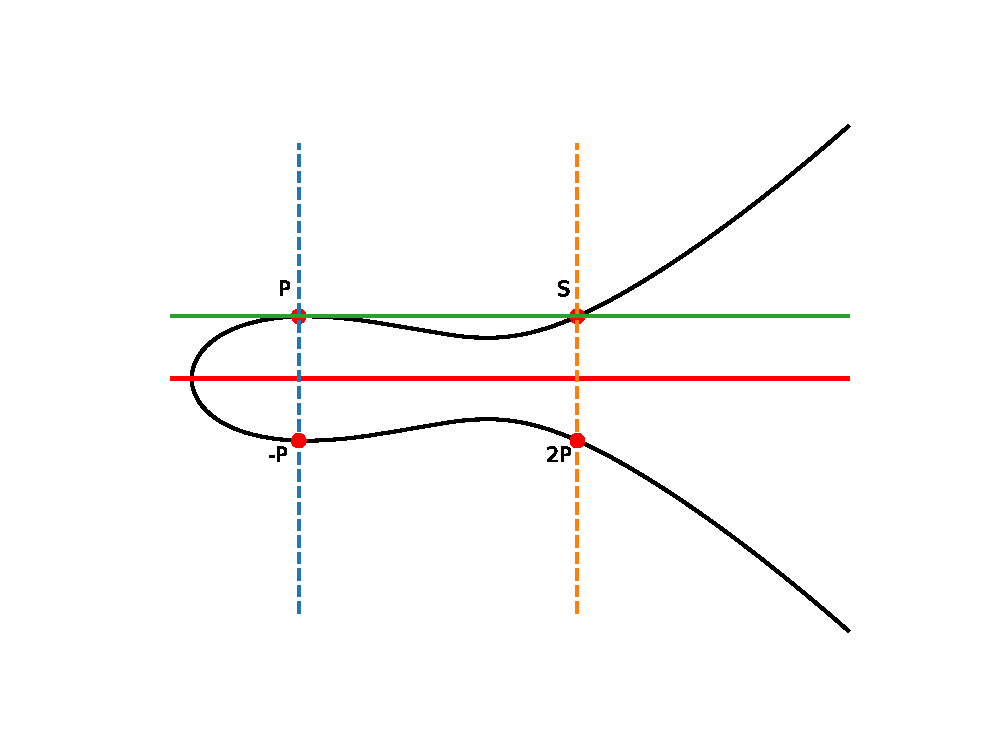
\includegraphics[width=8cm]{figures/elliptic1.eps}}}%
  %\caption{Cálculo de $2P$ y $-P$}
	\caption{Curva elíptica $y^2 = x^3 -3x + 5$}%
	\label{fig:test}%
\end{figure}
%incluir una figura
%\begin{figure}
%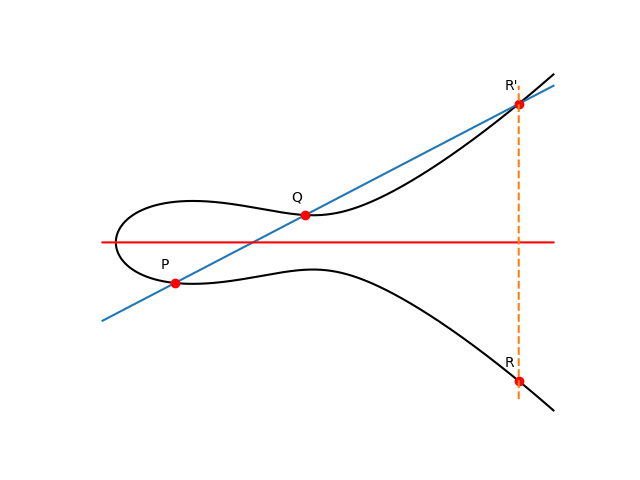
\includegraphics[height=2.9in]{figures/elliptic.png}
%\caption{Curva elíptica $y^2 = x^3 -3x + 5$}
%\end{figure}


A partir de la definición anterior de las operaciones no es difícil ver que el punto del infinito es el elemento neutro de la suma, que esta operación de suma es conmutativa y que existe el inverso de todo elemento. Sin embargo que la suma está cerrada con esta definición y que se cumple la propiedad asociativa no son resultados inmediatos. Una prueba de esto se puede consultar en \citep{group_law} y en \citep{group_law_verrill} 
%http://www.math.ku.dk/~kiming/lecture_notes/2000-2001-elliptic_curves/grouplaw.pdf 

Al cumplirse las cuatro propiedades anteriores tenemos que la suma así definida induce un grupo abeliano sobre los puntos de la curva elíptica. Sea $(G,+)$ este grupo y $n=|G|$ su orden. Sabemos que $n$ no es infinito pues la curva está definida sobre $\mathbb{K}$ un cuerpo finito, y por tanto sus puntos vendrán dados por $\{(x,y)| y^2 \equiv x^3 + ax + b  (mod  p) \}$. 
\theoremstyle{theorem}\begin{theorem}[Teorema de Cauchy]\label{cauchy} Sea G un grupo finito y q un primo. Si q divide al orden de G entonces existe un elemento de G de orden q.
\end{theorem}
Tenemos por tanto un grupo finito, donde a consecuencia del Teorema de Cauchy para grupos \ref{cauchy} podemos encontrar un elemento de orden primo $q$ (si $n = |G|$ ya es primo basta tomar $q = n$) Este elemento $g$ de $G$ genera un subgrupo cíclico ($<q>$) que será sobre el que se definan los protocolos criptográficos que veremos.


%Un subgrupo cíclico tiene orden $q$ siendo $q$ un primo tal que que $q|n$. Si $n$ es primo decimos entonces que $|G|$ es un grupo cíclico. %meter teorema de cauchy para ver la existencia de este subgrupo ciclico
%Será sobre este subgrupo cíclico sobre el que se definan los protocolos criptográficos que veremos.

\section{Funciones Hash}\label{hash}
Antes de ver el algoritmo ECDSA hay que definir el concepto de función hash y ver alguna de sus propiedades.
\theoremstyle{definition}\begin{definition}[Función Hash]\label{hash_def} Una función hash es una aplicación $\textit{H}$ entre cadenas tal que su conjunto imagen está formado por cadenas de longitud fija, siendo esta magnitud la longitud hash de la función, mientras que su preimagen está formada por cadenas de longitud arbitraria. Se escribe entonces $\textit{H}: \{0,1\}^* \rightarrow \{0,1\}^n$ si hablamos de cadenas de bits y denotamos por $n$ a la longitud hash de $\textit{H}$.\end{definition}

Aunque se hable de longitudes arbitrarias pueden existir limitaciones técnicas en cuanto a la longitud del mensaje de entrada. Considerando por ejemplo la función hash SHA-256 (SHA son las siglas de Secure Hash Algorithm) usada ampliamente en diferentes implementaciones del protocolo blockchain, que devuelve cadenas de 256 bits \citep{sha256_2}. Tenemos que esta función hash puede procesar mensajes de un máximo de $(2^{64} -1)$ bits \citep{sha256}. Es decir, que no se puede obtener el valor de hash de esta función para ninguna cadena que supere esa longitud, pero teniendo en cuenta que este valor equivale a más de 2 millones de terabytes esto no supone un verdadero problema en la práctica.

Una primera consecuencia de la definición \ref{hash_def} es que la preimagen de una función hash tiene cardinal estrictamente mayor que su imagen. Por tanto, por el principio del palomar, tendremos que si $A$ es el conjunto preimagen de cierta función hash $H$ y $B$ es su imagen para todo $b \in B$  $\exists \{a_{1},a_{2}\}$ con $a_{i} \in A$ distintos tales que $H^{-1}(b) = a_i$. Este fenómeno se llama colisión y se define en la resistencia a colisiones de una función hash como la probabilidad de encontrar un par $(a_{0},a_{1})$ con $a_{0} \not= a_{1}$ tales que se cumpla  $H(a_{0}) = H(a_{1})$. A toda función hash $H$, que usemos en el protocolo blockchain o en el algoritmo ECDSA, le pediremos que ningún algoritmo pueda encontrar una colisión para $H$ en tiempo polinómico, en este caso diremos que $H$ es resistente a colisiones. Otras dos propiedades importantes de las funciones hash serán la resistencia a preimágenes y a segundas preimágenes. La primera de estas propiedades viene a decir que debe ser \textit{díficil} dado un $b$ en el espacio de llegada encontrar un $a$ en el espacio de partida tal que $H(a) = b$. La segunda propiedad es similar a la definición de resistencia a colisiones, dado un $a_{0}$ elegido de forma aleatoria debe ser \textit{díficil} encontrar un $a_{1}$ distinto de $a_{0}$ tal que $H(a_{0}) = H(a_{1})$. Esta noción de \textit{difícil} viene dada por la imposibilidad de resolver en tiempo polinómico cualquiera de estos problemas.

La propiedad de resistencia a segundas preimágenes es  más fuerte que la resistencia a colisiones como consecuencia de la paradoja del cumpleaños. En efecto, si suponemos cadenas binarias y una longitud hash de $n$ nuestra función devolverá exactamente $2^{n}$ cadenas distintas. Dadas $l$ cadenas elegidas al azar la probabilidad de no encontrar una colisión viene dada por:
\begin{equation}
NC(2^{n},l) = \frac{2^{n}}{2^{n}}\frac{2^{n}-1}{2^{n}}\ldots\frac{2^{n}-(l-2)}{2^{n}}\frac{2^{n}-(l-1)}{2^{n}} = \prod_{i=0}^{l-1}(1-\frac{i}{2^{n}})
\end{equation} 
Así que la probabilidad de encontrar una colisión $C(2^{n},l)$ será su complementario:
\begin{equation}
C(2^{n},l) = 1-\prod_{i=0}^{l-1}(1-\frac{i}{2^{n}})
\end{equation}
Considerando que el cociente $i/2^{n}$ es cercano a cero, que es consecuencia de tomar $n$ suficientemente grande, y teniendo en cuenta que la expansión en Serie de Taylor de $e^{x}$ se puede truncar a partir del término cuadrático para $x \ll 1$. Tenemos que:
\begin{equation}
C(2^{n},l) \approx 1- \prod_{i=0}^{l-1}\exp\left(\frac{-i}{2^{n}}\right) = 1- \exp\left(\sum_{i=0}^{l-1}\frac{-i}{2^{n}}\right)
\end{equation} 
Este último sumatorio se puede escribir como $-(l-1)l/2^{n+1}$ usando la fórmula de la suma de los $(l-1)$ primeros naturales. Y que para $l$ suficientemente grande se puede aproximar a $-l^{2}/2^{n+1}$.
Tomando logaritmos y despejando se tiene que:
\begin{equation}
l \approx 2^{n/2}\sqrt{-2\log(1-C(2^{n},l))}
\end{equation}
Si se considera una probabilidad $C(2^{n},l) = 0.5$, es decir que de un total de $2^{n}$ elementos distintos la probabilidad de encontrar en un grupo de $l$ elementos elegidos al azar al menos 2 iguales es del $50\%$  entonces se tiene que $\sqrt{-2\log(1-C(2^{n},l))}\approx 1.18$. Así  $l \approx 1.18*2^{n/2}$, que es el número mínimo de cadenas binarias necesarias para garantizar una colisión con una probabilidad del $50\%$


 Sin embargo, la probabilidad de encontrar una segunda preimagen comprobando solo $1.18\sqrt{2^{n}}$ cadenas es de 
 \begin{equation}\label{preimagen_eq}
\frac{1.18\sqrt{2^{n}}}{2^{n}} = \frac{1.18}{2^{n/2}}
\end{equation}
Para $n > 20$ la probabilidad anterior prácticamente cero (En la función SHA-256 se tiene que $n = 256$).

Para garantizar una probabilidad de encontrar una preimagen de al menos el 0.5 se tiene que el número de k de cadenas a comprobar debe ser de al menos:
\begin{equation}
k=\frac{1}{2}2^{n} = 2^{n-1}
\end{equation}
Donde se ha utilizado, al igual que en \ref{preimagen_eq}, la \textit{Regla de Laplace} (Número de casos favorables entre Número de casos posibles).  Como se ve, para n suficientemente grande el coste de encontrar una preimagen es prácticamente el mismo que el de comprobar todas las posibles cadenas que produce nuestra función hash.

Tomando $2^{n} = 365$, es decir, ahora el número de casos posibles es 365 (ya no estamos mirando cadenas binarias) se obtiene el problema del cumpleaños: para garantizar una colisión (dos individuos que cumplan años el mismo día) con una probabilidad de al menos $50\%$ basta con reunir 23 personas, este resultado es mucho menor que el valor que podríamos dar intuitivamente, de ahí que se le llame paradoja aunque desde el punto de vista estrictamente lógico no lo sea.


Hay que señalar que los cálculos anteriores solo son válidos bajo ciertos supuestos teóricos que en la práctica no se dan, pues ninguna función hash lleva los elementos del espacio de partida al de llegada siguiendo patrones completamente aleatorios. Una vez han sido encontradas colisiones (o se ha probado que la probabilidad de encontrarlas es \textit{alta}) la función hash deja de ser considerada segura. Un ejemplo de función hash en esta categoría es SHA-1, para la que se conocen colisiones desde 2017 \citep{sha-1}, aunque era considerada insegura desde 2005. 
La función hash que usaremos (SHA-256) es considerada segura por el momento.


%Referencias: http://web.cs.ucdavis.edu/~rogaway/papers/relates.pdf
%https://www.esat.kuleuven.be/cosic/publications/article-1532.pdf
%https://eprint.iacr.org/2004/304.pdf


%En el Bitcoin se usa en diferentes tareas la función hash SHA-256.

%trabajar esto algo mas



%una vez vista las operaciones que definen un grupo sobre la curva, especificar el algoritmo ecdsa. Luego de eso exponer el coste computacional de este algoritmo en todos los sentidos, usarlo como punto a favor del uso de curvas elipticas en lugar de logaritmos discretos u otros metodos.
\section{Algoritmo ECDSA}
%Referencia (además del libro) https://pdfs.semanticscholar.org/c06a/d6512775be1076e4abd43e3f2928729da776.pdf
%https://www.ietf.org/rfc/rfc6979.txt

Ahora podemos especificar el algoritmo ECDSA (Elliptic Curve Digital Signature Algorithm)\citep{elliptic_cripto}, tanto el usado para la firma de mensajes como el correspondiente algoritmo de verificación. Este algoritmo se basa en la dificultad computacional de resolver el problema del logaritmo discreto para curvas elípticas (ECDLP).

\theoremstyle{definition}\begin{definition}[Problema del logaritmo discreto para curvas elípticas]\label{ecdlp} Sea $E(\mathbb{K})$ una curva elíptica sobre un cuerpo $\mathbb{K}$. Sea $P \in E(\mathbb{K})$ y $Q  \in  <P>$. Encontrar $k$ tal que $Q= kP$. \end{definition}

La definición anterior tiene sentido pues como se vio en \ref{curvas_grupo} los puntos de una curva elíptica definida sobre un cuerpo finito forman un grupo y por tanto se puede hablar del grupo generado por cualquier elemento la curva. Así, se tiene que $<P>$ es el subgrupo cíclico generado por el punto $P$ de la curva $E(\mathbb{K})$. 

No se conoce algoritmo que resuelva este problema en tiempo subexponencial \citep{discrete_log}. Sin embargo, aunque aquí no serán especificados se necesitan algoritmos apropiados para crear y representar el cuerpo finito $\mathbb{F}_{p}$ de forma que se garantice la intratabilidad de este problema.
%El orden de una curva elíptica $E$ sobre un cuerpo finito $\mathbb{F}_{p}$ (número de puntos) es importante para garantizar la seguridad de este algoritmo.

Antes de poder firmar un mensaje hay que generar las claves públicas y privada.
Sea $P = (x_{1},y_{1})$ un punto de la curva elíptica $E(\mathbb{F}_{p})$ que genera un subgrupo cíclico $<P>$ de orden primo $n$. El par $(d,Q)$ de claves privada y pública se genera usando el algoritmo \ref{alg:claves}. La elección aleatoria de $d$ es muy importante, en otro caso se pueden tener problemas de seguridad que permitan encontrar la clave privada utilizada.
%no encontré buenas referencias sobre el hack de fail0verflow)
\begin{algorithm}
\caption{Generación de claves}\label{alg:claves}
\begin{algorithmic}[1]

\State Se elige $d \in [1, n-1]$ de forma aleatoria

\State Se calcula $Q=dP$

\State  $Q$ es la clave pública y $d$ la clave privada.
\end{algorithmic}
\end{algorithm}


Una vez se ha generado la clave privada y utilizando una función hash $H$ que devuelva cadenas de longitud menor o igual que $n$ se pueden firmar mensajes usando el algoritmo \ref{alg:firmar}
\begin{algorithm}[H]
\caption{Generación de firma}\label{alg:firmar}
\begin{algorithmic}[1]
\Repeat
\State Se elige $k \in [1, n-1]$ de forma aleatoria
\State Se calcula $z_{1} = kx_{1}$ 
\State Se calcula  $r = z_{1}  \mod n$ si $r = 0$ paso 1.
\State Se calcula $e = H(m)$
\State Se calcula $s = k^{-1}(e + dr)  \mod n$. Donde $k^{-1}$ es el inverso de k en el grupo $<P>$
\Until{$s \neq 0$}
\State Se devuelve $(r,s)$
\end{algorithmic}
\end{algorithm}

Ahora, quien recibe un mensaje $m$ con la firma $(r,s)$ puede verificar su procedencia (suponiendo que ha recibido antes la clave pública $Q$) mediante el algoritmo \ref{alg:verificar}

\begin{algorithm}
\caption{Validación de firma}\label{alg:verificar}
\begin{algorithmic}[1]
\State Verificar que $r,s \in [1, n-1]$, en otro caso \textbf{se rechaza la firma}
\State Se calcula $e = H(m)$
\State Se calcula $w = s^{-1}  \mod n$
\State Se calcula $u_{1} = ew  \mod n$, $u_{2} = rw  \mod n$
\State Se calcula $X = u_{1}P + u_{2}Q$, si $X=\infty$ \textbf{se rechaza la firma} \Comment{$X \in E(\mathbb{F}_{p})$}
\State Sea $X = (x_{1},y_{1})$, se calcula $v = x_{1} \mod n$
\State Si $v = r$ \textbf{se acepta la firma}, en otro caso \textbf{se rechaza la firma}
\end{algorithmic}
\end{algorithm}

La importancia de la resistencia a colisiones en la función hash $H$ queda explicada con los algoritmos anteriores.
La existencia de colisones conocidas (o facilmente calculables) hace que ya no sea posible garantizar la validez de una firma. Un atacante podría usar un mensaje firmado, buscar alguna modificacion de este mensaje que combinada con la firma devuelva el mismo valor hash que en el original. Ahora quien verifique este mensaje falso seria incapaz de distinguirlo del original.

%(Poner imagen de https://shattered.it/ como ejemplo de colision)

%mirar https://webusers.imj-prg.fr/~ricardo.perez-marco/blockchain/BitcoinP7.pdf en los referente a hash